%\documentclass[
%11pt, % The default document font size, options: 10pt, 11pt, 12pt
%%oneside, % Two side (alternating margins) for binding by default, uncomment to switch to one side
%%chapterinoneline,% Have the chapter title next to the number in one single line
%english, % ngerman for German
%singlespacing, % Single line spacing, alternatives: onehalfspacing or doublespacing
%%draft, % Uncomment to enable draft mode (no pictures, no links, overfull hboxes indicated)
%%nolistspacing, % If the document is onehalfspacing or doublespacing, uncomment this to set spacing in lists to single
%%liststotoc, % Uncomment to add the list of figures/tables/etc to the table of contents
%%toctotoc, % Uncomment to add the main table of contents to the table of contents
%%parskip, % Uncomment to add space between paragraphs
%%nohyperref, % Uncomment to not load the hyperref package
%headsepline, % Uncomment to get a line under the header
%]{MastersDoctoralThesis} % The class file specifying the document structure
%
%\usepackage[utf8]{inputenc} % Required for inputting international characters
%\usepackage[T1]{fontenc} % Output font encoding for international characters
%\usepackage{graphicx}
%\usepackage{aas_macros}
%\usepackage{amsmath}
%\usepackage{amssymb}
%\usepackage[authoryear]{natbib}
%%\usepackage{hyperref}
%\usepackage[colorlinks]{hyperref}
%\usepackage{palatino} % Use the Palatino font
%
%
%\hypersetup{linktocpage} % For linking the bookmarks to page numbers in Tables of Contents, Figures, Tables, Publications etc.
%
%\hypersetup{colorlinks,linkcolor=blue}
%
%
%\begin{document}























\global\long\def\fsc{\alpha_f}
\global\long\def\ee{E_0}

I note here that the work described in this chapter is based on \textbf{[Zdziarski, Paul \& Rao, 2016]}, carried out in collaboration with Professor Andrzej Zdziarski, Nicolaus Copernicus Astronomical Center (NCAC), Warsaw. I am indebted to the hospitality provided to me by Professor Andrzej Zdziarski for my visit to NCAC for 4 days in the month of June, 2016, supported by the Polish National Science Center grant provided by the Polish Academy of Sciences.

\section{Introduction}

The discovery of double-lobed radio sources via imaging carried out by radio telescopes \citep{MacDonald_et_al.-1968-MNRAS,Mackay-1969-MNRAS,Branson_et_al.-1972-MNRAS,Hargrave-1974-MNRAS, Hargrave_&_Ryle-1974-MNRAS,Fanaroff_&_Riley-1974-MNRAS}, and their interpretation in terms of extragalactic relativistic jets \citep{Longair_et_al.-1973-MNRAS,Blandford_&_Rees-1974-MNRAS,Scheuer-1974-MNRAS}, opened up a new field, which still has a number of open questions (for an early review, see \citealt{Begelman_et_al.-1984-RevModPhys}). Highly resolved imaging of these sources with the advent of very long baseline interferometry has truly revolutionized the field \citep{Biretta_et_al.-1986-ApJ,Marscher-1988-ApJ,Reid_et_al.-1989-ApJ}, the observations opening up many more questions than can be answered by the most advanced theories. More recently, the discovery of `Microquasars' \citep{Mirabel_&_Rodriguez-1992-Nature,Mirabel_&_Rodriguez-1994-Nature,Mirabel_&_Rodriguez-1998-Nature} has added jets from black hole binary systems to the existing list, and has led to the firm conclusion that these are highly collimated relativistic \citep{Ryle_&_Longair-1967-MNRAS,Blandford_et_al.-1977-Nature} ejecta of matter from the neighbourhood of a central object, in most cases a black hole, accreting matter from its surroundings.

The earliest theoretical studies to explain the observed properties of relativistic jets \citep{Blandford_&_Rees-1974-MNRAS,Blandford_&_McKee-1976,Blandford_&_McKee-1977-MNRAS,Blandford_&_Konigl-1979-ApJ,Lind_&_Blandford-1985-ApJ} identified the observed electromagnetic radiation to be non-thermal emission from the relativistic particles in the jet, specifically synchrotron radiation in the presence of magnetic fields in the black hole environment. In the \citealt{Blandford_&_Konigl-1979-ApJ} model, it is proposed that a steady jet, fed by a central engine, powers the radio emission, whereas the variability in the observed flux are produced behind strong shocks that either transmit along the jet or are produced at the termination of the jets. Here the authors investigate the properties of synchrotron radiation emitted by a population of non-thermal plasma, and conclude that the observed spectrum may be flat, i.e. the `spectral index',
\begin{equation}
\alpha = \frac{d (\ln F)}{d (\ln E)}
\end{equation} (where $ F $ is the flux per unit energy, $ E $) will be $ 0 , $ if the jet is partially self-absorbed at radio wavelengths.

In Microquasars such as GRS 1915+105 \citep{Fender_et_al.-1999-MNRAS}, Cygnus X-3 \citep{Miller-Jones_et_al.-2004-ApJ}, very long baseline interferometry radio images have shown evidence of discrete blobs moving away from a central source at apparent superluminal speeds \citep{Dhawan_et_al.-2000-ApJ}, generally associated to the ejection of the `corona' in the soft spectral state \citep{Fender_et_al.-2004-MNRAS}. In the case of Microquasars like Cygnus X-1 \citep{Russell_&_Shahbaz-2014-MNRAS}, the jet appears to be steady
over time-scales of a few days. This might be attributed to the steady replenishment of fresh relativistic particles by the 'central engine' driving the jet, the details of which are not considered.

In this chapter, we revisit the findings of the \citealt{Blandford_&_Konigl-1979-ApJ} model. Specifically, we investigate the dependence of the observed flux from steadily replenished synchrotron jets, on its Doppler-factor, and the jet-viewing angle, see below. The authors of the above paper do not take into account these dependencies in the case of partially optically thick, i.e. partially self-absorbed, jets. For conical jets, they limit the discussion to the jet viewed from the side in the comoving frame of reference, a limitation that we address. In our study, magnetic fields play a passive role, and we do not consider the origin of these fields.

In Section \ref{sec:the_model}, we describe the salient features of the model considered. In Section \ref{sec:flux_calculation}, we carry out the radiative transfer calculations to calculate the observed flux at various approximate viewing angles. In Section \ref{sec:comparison}, we make a comparative study of the fluxes at different angles and in Section \ref{sec:jet-to-counterjet_ratio}, calculate the jet-to-counterjet flux-ratio. In Section \ref{sec:CygX-1}, we apply our findings to a known astrophysical system, and conclude our studies in Section \ref{sec:conclusions}. We finally carry out a discussion of the limitations and future directions in Section \ref{sec:discussions}.


\section{The model} \label{sec:the_model}

Here we adopt the model of \citealt{Zdziarski_et_al.-2012-MNRAS-MeV_tail_CX1}. The jet consists of electrons moving with a bulk or average speed $ v = c \, \beta_j \; (c $  is the speed of light in vacuum) along a certain direction, which defines the `jet-axis' and makes an angle $ i $ to our line of sight. The height from the black hole in the observer's frame is denoted by $ h, $ parametrized by
\begin{equation}
\xi = h / h_0 \label{eq:xi_definition}
\end{equation}
where $ h_0 $ defines the `jet-base' as follows. In this model, the electrons are assumed to have been accelerated and collimated along the jet-axis below $ h_0 , $ through mechanisms that are not considered. Thus effectively $ h_0 $ defines a transition between an `acceleration region' with which we will not be concerned and the `emission region' which is our region of interest.

Although electrons move along the jet with bulk Lorentz factor
\begin{equation}
\Gamma_j = \left(1-\beta_j^{2}\right)^{-1/2},
\end{equation} the energy-distribution of the population is assumed to be non-thermal, specifically a power-law in the Lorentz-factor $ \gamma $ and index $ p , $ such that the number-density $ N \left(\gamma\right) $ is defined by 
\begin{equation}
N \left(\gamma\right) = K\,\mathrm{\gamma^{-p}}, \; p > 1 \label{eq:energy-distribution}
\end{equation}
where $ K $ is the normalization. This electron population gyrates about magnetic fields frozen in the system as they coast along the jet, losing a small fraction of their energy into synchrotron radiation which we observe. We assume a conical jet with a half-angle of $ \theta_j , $ and the width of the cone at the jet-base is neglected assuming the jet is launched from a region only a few gravitational radii wide. The electron distribution is assumed to be maintained by the mechanism that produces the bulk energy of the jet. This is consistent with the observations of steady radio emission up to $ \sim \mathrm{AU} $ length-scales in Microquasars. The study of \citealt{Russell_&_Shahbaz-2014-MNRAS} support the general features of this model for the Microquasar Cygnus X-1. We do not consider the variation of $ \Gamma_j $ along the jet due to adiabatic cooling or radiative losses and the subsequent variation of the electron energy as a function of $ h, $ which are ultimately responsible for the termination of the jet.

Following \citealt{Blandford_&_Konigl-1979-ApJ}, we assume conservation of the electron number distribution along the jet, which lets us write
\begin{equation}
K = K_0 \, \xi^{-2}. \label{eq:K}
\end{equation}
We also assume conservation of the energy flux in toroidal or tangled magnetic field,
\begin{equation}
B = B_0 \, \xi^{-1}. \label{eq:B}
\end{equation}

We introduce the label $ n $ for the jet $ (j) $ or counter-jet $ (cj) . $ For example, we adopt $ \delta $ for the Doppler factor and hence $ \delta_{j} $ and $ \delta_{cj} $ stand for the Doppler factor for the jet and the counter-jet respectively, while $ \delta_{n} $ stands for either. Thus,
\begin{equation}
\delta_j = \dfrac{1}{\Gamma \left( 1 - \beta\mathrm{\,cos}i\right) },\label{eq:Doppler_factor_for_jet}
\end{equation} and
\begin{equation}
\delta_{cj} = \dfrac{1}{\Gamma \left( 1 + \beta\mathrm{\,cos}i\right) }.\label{eq:Doppler_factor_for_counterjet}
\end{equation}
We also define \begin{equation}
w \equiv \frac{\delta_{cj}}{\delta_{j}} = \dfrac{1 - \beta\mathrm{\,cos}i}{1 + \beta\mathrm{\,cos}i} \label{eq:w}
\end{equation} and note that $ w \leq 1, $ whereas $ w = 1 $ is the case when the jet and counter jet appear symmetrically on the plane of the sky, i.e. $ i = 90^{0}. $

In this work, we generalize the application of the jet model to extragalactic jets, and hence consider the redshift of the system, $ z, $ and consider the distance to the system is considered to be the luminosity distance, given by $ D. $ We write the observed energy of the emitted photons, $ E, $ in terms of dimensionless form $ \epsilon $ in the co-moving (jet/counter-jet) frame,
\begin{equation}
\epsilon_{n} = \frac{ (1+z) E }{ \delta_{n} \, \ee }, \label{eq:epsa_n}
\end{equation} where $ \ee $ is the rest-energy of electron. We assume that the synchrotron cooling break is well above the interested energy-regime, and hence do not consider it.

We assume that the jet and the counter-jet are symmetric in the co-moving frame, since there is no compelling observational reason to assume otherwise. We also assume that the synchrotron emission in the local frame is isotropic. This is justified if the magnetic field is tangled. Hence, we adopt the expressions for the pitch-angle averaged emission co-efficient $ j \left( \epsilon \right) $ and absorption co-efficient $\alpha(\epsilon)$ for synchrotron emission from power-law electrons in the CGS system, given by \citep{Longair-3rd_Ed.,Zdziarski_et_al.-2012-MNRAS-MeV_tail_CX1},

\begin{equation}
j(\epsilon) = cB_{cr}^{2} \frac{C_1(p) \sigma_T K}{48\pi^2}\left(\frac{B}{B_{cr}}\right)^{\frac{p+1}{2}} \epsilon^{\frac{1-p}{2}}\label{eq:emission_coefficient}
\end{equation}
and
\begin{equation}
\alpha(\epsilon) = \frac{\pi C_2(p) \sigma_T K}{2 \fsc}\left(\frac{B}{B_{cr}}\right)^{\frac{p+2}{2}} \epsilon^{-\frac{p+4}{2}} \equiv \alpha_0 \, \xi^{-\frac{p+6}{2}} \epsilon^{-\frac{p+4}{2}}, \label{eq:absorption_coefficient}
\end{equation}
where $ B_{cr} = \frac{\ee^2}{c e \hbar} , \; e $ is the electronic charge, $ \hbar $ is the reduced Planck's constant,
\begin{equation}
C_1(p) = \dfrac{ 3^{\frac{p+4}{2}} \Gamma(\frac{3p-1}{12}) \Gamma(\frac{3p+19}{12}) \Gamma(\frac{p+1}{4}) }{ 2^5 \pi^{1/2} \Gamma(\frac{p+7}{4}) }, \label{eq:C_1}
\end{equation}

\begin{equation}
C_2(p) = \dfrac{ 3^{\frac{p+3}{2}} \Gamma(\frac{3p+2}{12}) \Gamma(\frac{3p+22}{12}) \Gamma(\frac{p+6}{4}) }{ 2^4 \pi^{1/2} \Gamma(\frac{p+8}{4}) }, \label{eq:C_2}
\end{equation}
and
\begin{equation}
\alpha_0 \equiv  \frac{\pi C_2(p) \sigma_T K_0}{2 \fsc}\left(\frac{B_0}{B_{cr}}\right)^{\frac{p+2}{2}}. \label{eq:alphazero}
\end{equation}

These equations define the source function,
\begin{equation}
S(\epsilon, \xi) \equiv \frac{j}{\alpha} = \dfrac{\fsc C_1(p) c B_{cr}^{5/2}}{24 \pi^2 C_2(p) B_0^{1/2}} \, \epsilon^{5/2} \xi^{1/2} \equiv S_0 \, \epsilon^{5/2} \xi^{1/2} , \label{eq:source_function}
\end{equation} where
\begin{equation}
S_0 \equiv \dfrac{\fsc C_1(p) c B_{cr}^{5/2}}{24 \pi^2 C_2(p) B_0^{1/2}}. \label{eq:Szero}
\end{equation}


\begin{figure}
\noindent \centering{}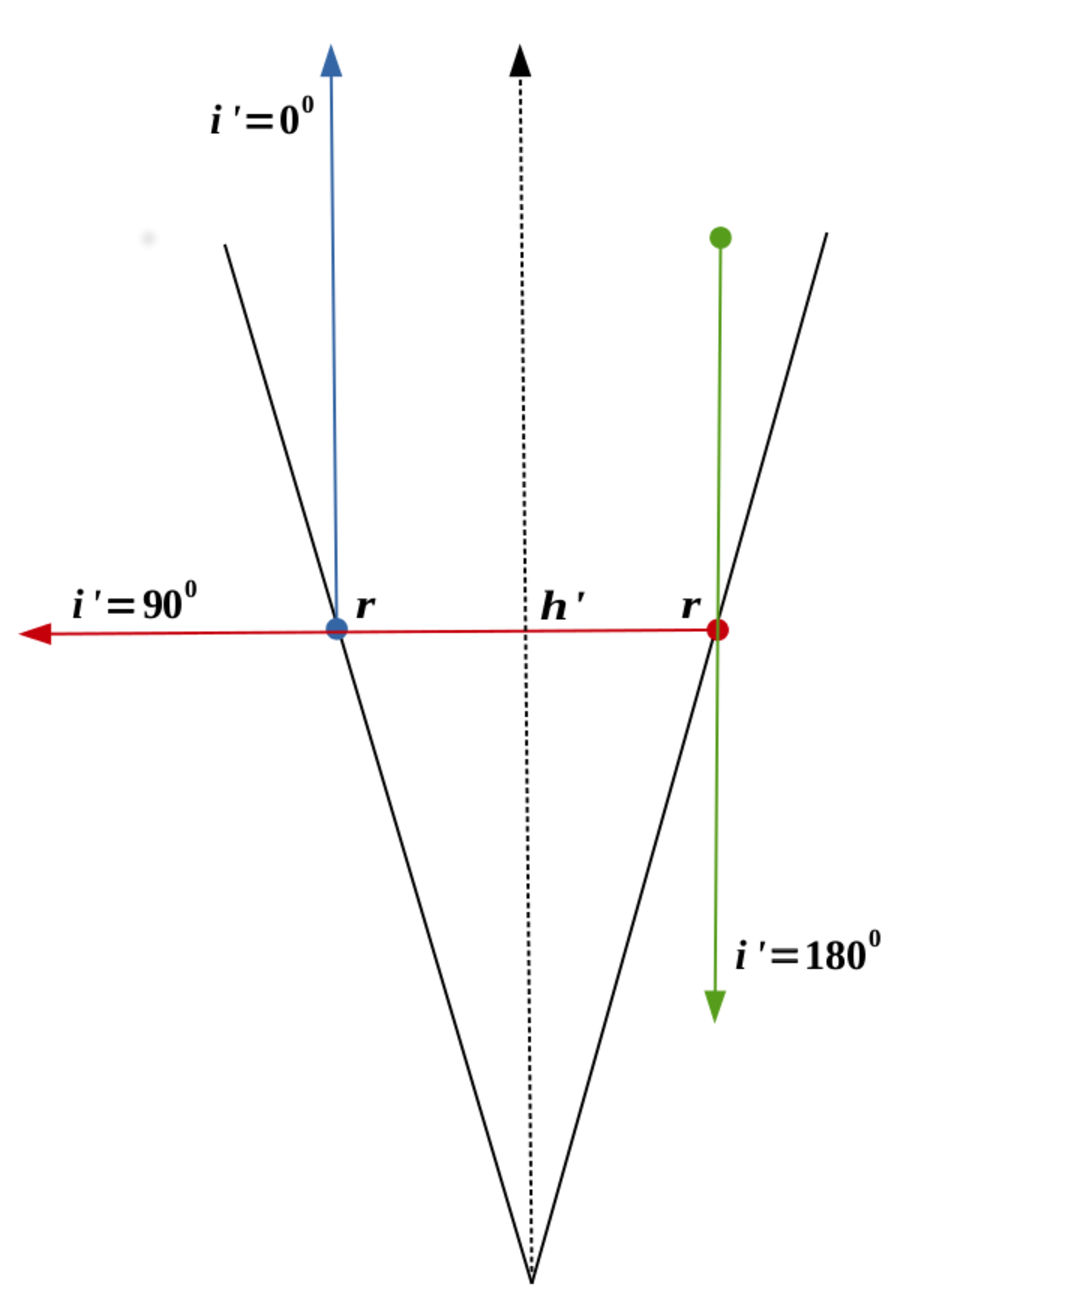
\includegraphics[scale=0.68]{emission_angles.pdf}\caption{A schematic drawing of the jet and photon paths in the co-moving frame. We show three cases of the photon path: (i) perpendicular to the jet axis, in red, (ii) along the jet axis and in the direction of the jet motion, in blue, and (iii) along the jet axis backward, in green. The beginning of the photon paths are marked by the filled circles. The intersections of the photon path with the jet boundary are at the vertical distance $ h $ from the origin and $ h' $ in the co-moving frame, and at the radial distance $ r = r' $ from the jet axis. Note that the co-moving frame is not stationary, i.e. $ h' $ and $ r $ increase with time.}
\label{fig:The_emission_angles}
\end{figure}


\section{The flux from the jet and the counterjet} \label{sec:flux_calculation}

The observed synchrotron flux from the jet can be obtained by solving the radiative transfer equation over the line-of-sight, and then transforming to the observer's frame. In general, this can be obtained only numerically in the conical geometry. Below we consider two limiting cases.


\subsection{Viewed from the side}


If the observing angle is large, we can neglect the variation of $ K $ and $ B $ over the line-of-sight. In particular, if $ \sin i \sim \frac{1}{\Gamma_j} , $ the emission angle in the co-moving frame is, $ i' \sim 90^{\circ} , $ which follows from the conservation of photon momentum in a direction perpendicular to the relative motion between the two frames,
\begin{equation}
\frac{E}{c} \sin i = \frac{E'}{c} \sin i',
\end{equation}
and using the transformation of energy between the two frames,
\begin{equation}
E = \delta_j E',
\end{equation}
giving
\begin{equation}
\sin i' = \delta_j \sin i.
\end{equation}


\begin{figure}
\noindent \centering{}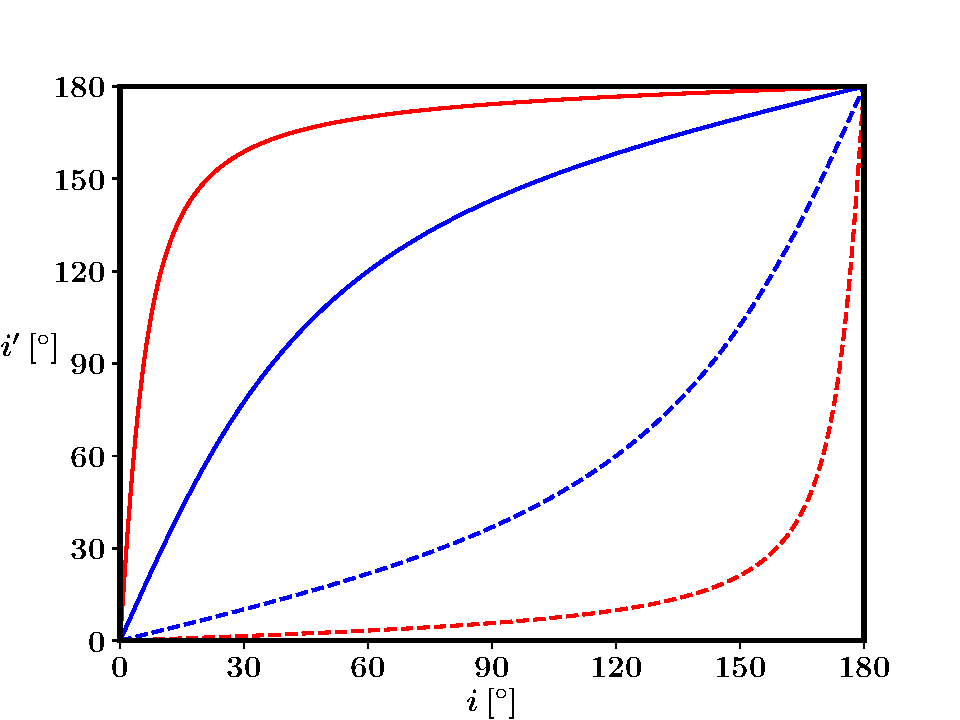
\includegraphics[scale=0.40]{angle_transformation.pdf}\caption{{The effect of the special relativistic transformation on the emission angle in the observer frame, $ i $. The angles in the co-moving frame, $ i' $, are shown for the jet and counterjet by the solid and dashed curves, respectively. The blue and red curves are for $ \Gamma_j = 5/3 \, ( \beta_j = 0.8 ) $ and $ 10 \, ( \beta_j = 0.995 ) , $ respectively. We see that at large $ \Gamma_j $, the jet-frame viewing angle for most values of $ i $ is close to $ 180 ^ {\circ} $.}
\label{fig:The_angle_transformation}}
\end{figure}


In Fig. \ref{fig:The_angle_transformation}, we show the transformation for fiducial values of $ \beta_j . $ We note that viewing angles in the co-moving, $ i' \gg 90 ^{\circ} $ for most viewing angles in the observer's frame, $ i \gtrsim 40^{\circ} $ even for mildly relativistic cases. This means that the photons which are moving at obtuse angles to the observer's line-of-sight in the co-moving frame, are actually directed towards the observer because of the relativistic bulk motion. This effect, though generally not mentioned, has no counterparts in classical mechanics. We also note from the dashed curves that the counterjet emission for small viewing angles is actually produced by the counterjet photons moving in the direction towards the jet-base in the co-moving frame. This effect will be considered later.

Within the above-mentioned large-angle approximation, see Case (ii) in Fig \ref{fig:The_emission_angles}, it is justified to assume the source function to be constant along the line-of-sight, for which the specific intensity $ I $ solves to $ S [ 1 - \exp(-\tau) ],  $ where $ \tau $ is the integrated optical depth along the line-of-sight, see for example Equation (1.29) of \citealt{Rybicki_&_Lightman}. Then the observed flux is given by integrating the specific intensity over the projected area of the source and then transforming to the observer's frame (both boost and cosmological expansion are considered),
\begin{equation}
F_{n} (i' \sim 90^{\circ}) = \frac{ (1+z)\delta_n^{3} \sin i }{ \ee\, D^2 } \, \intop_{h_0}^{\infty} dh \, S(h) \, \int_{-h \ \tan \theta}^{+h \, \tan \theta} dx \, [1 - \exp(-\tau)],
\label{eq:Flux-n_beginning}
\end{equation} where the $ x $-axis is defined to lie on a plane perpendicular to the line-of-sight and the $ h $-axis. The assumption that the jet extends to $ \infty $ is justified because the uppermost parts of the jet contribute negligibly to the emission.

The integrated optical depth is given by \citep{Heinz-2006-ApJ,Zdziarski_et_al.-2012-MNRAS-MeV_tail_CX1},
\begin{eqnarray}
\tau & = & \dfrac{2 \, \alpha(\epsilon) \, \sqrt{ (h \tan \theta)^{2} - x^2 }  }{ \delta_j \sin i } \label{eq:optical_depth_side_view_1} \\
i.e., \; \tau( \epsilon, \xi, \psi ) & = & \frac{2 h_0 \tan \theta}{\sin i}(1-\psi^{2})^{1/2} \,\frac{\alpha(\epsilon) \xi}{\delta_{n}} , \label{eq:optical_depth_side_view_2}
\end{eqnarray} where
\begin{equation}
\psi = \frac{x}{h \tan \theta}. \label{eq:psi}
\end{equation}

We mathematically define the `jet-base' such that
\begin{equation}
\tau\left( \epsilon_{t}, \, 1, \, 0 \right) = 1, \label{eq:jet_base}
\end{equation}
i.e. the emission from the `turn-over' energy in the co-moving frame becomes optically thin at that height, along the jet-spine. Equations \ref{eq:absorption_coefficient}, \ref{eq:optical_depth_side_view_1} and \ref{eq:jet_base} can be combined to give
\begin{equation}
\frac{\epsilon_{t,cj}}{\epsilon_{t,j}} =  w^{-\frac{2}{p+4}} . \label{eq:jet_to_counterjet_turnover_ratio}
\end{equation}

We note that the turnover energies in the co-moving frame become equal in the limit $p\rightarrow\infty.$ Equations \ref{eq:epsa_n} and \ref{eq:jet_to_counterjet_turnover_ratio} are then combined
to give 
\begin{equation}
\quad\frac{E_{t,cj}}{E_{t,j}} = w^{\frac{p+2}{p+4}} . \label{eq:observed_turnover_ratio}
\end{equation}

This implies $ E_{t,cj} < E_{t,j} $ and hence the observed turnover energy is
\begin{equation}
E_{t} = E_{t,j}
\end{equation} above which the entire jet is optically thin, and below which the jet is partially optically 
thick.

\begin{figure}
\noindent \centering{}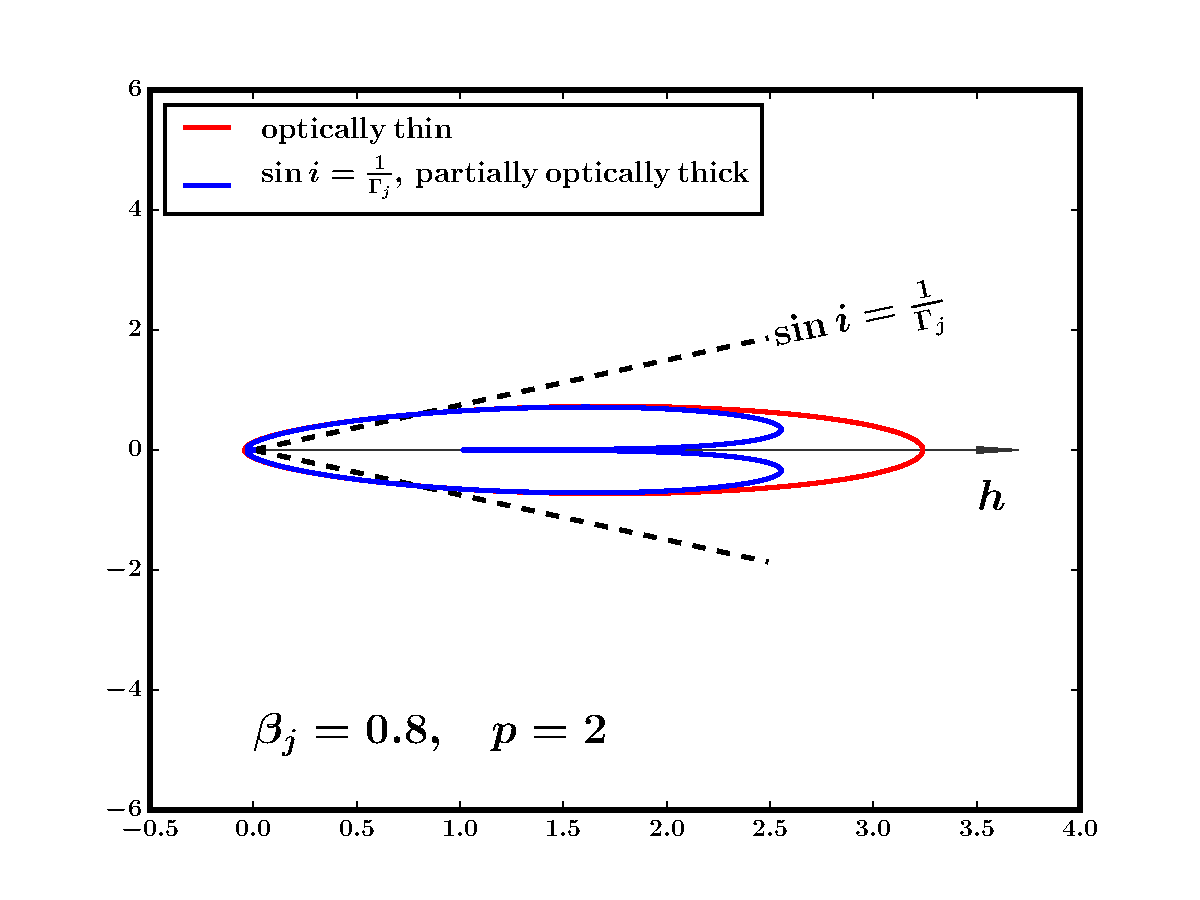
\includegraphics[scale=0.6]{beaming_initial.pdf}\caption{The beaming pattern of the partially optically thick flux, compared against a strictly optically thin emission, shown in a polar plot, for the fiducial parameters $ \beta_j = 0.8 $ and $ p = 2 . $ The flux is normalized to unity at $ \sin i = 1 / \Gamma_j , $ which is Case (ii) in Fig. \ref{fig:The_emission_angles}. It is seen that at low viewing angles, the flux sharply approaches zero, which we point out as unphysical.}
\label{fig:beaming_initial}
\end{figure}

Using Equations \ref{eq:optical_depth_side_view_2} and \ref{eq:jet_base}, we write,
\begin{equation}
\tau = (1-\psi^{2})^{1/2}\,\xi^{-\frac{p+4}{2}}, \label{eq:tau_to_integrate}
\end{equation} which finally allows us to write Equation \ref{eq:Flux-n_beginning} as

\begin{equation}
F_n (i' \sim 90^{\circ}) = (1+z) \dfrac{\fsc^{\frac{p-1}{p+4}} C_{1} C_{3} \left( \tan \theta_{j} \right)^{\frac{p+9}{p+4}} \; \delta_n^{\frac{3p+7}{p+4}} \left( \sin i \right) ^{\frac{p-1}{p+4}}}{24 \, \pi^{\frac{3p+7}{p+4}} C_{2} ^{\frac{p-1}{p+4}}} \left(\dfrac{\sigma_T h_0 K_0 B_{cr}}{B_0}\right)^{\frac{5}{p+4}} \frac{ c B_0{^2} }{\ee} \left(\frac{h_0}{D}\right)^2, \label{eq:Flux_side_view}
\end{equation} where we remind ourselves that $ C_1, \; C_2 \; $ depend on $ p, $ and
\begin{equation}
C_{3,n}(p, E) = \int_{\left(\frac{\epsilon}{\epsilon_{t}}\right)_{n}}^{\infty}d\xi\,\xi^{3/2}\,\int_{-1}^{1}d\psi\, \left[ 1 - \exp \left\{ -\xi^{-\frac{p+4}{2}}\left(1-\psi^{2}\right)^{1/2} \right\} \right]. \label{eq:C_3_double_integral}
\end{equation}

The lower-limit $ \epsilon / \epsilon_{t} $ justifies the subscript $ n $ on $ C_{3} . $ It reduces to $ E / E_{t} $ for the jet and $ \left(E/E_{t}\right) w^{ -\frac{p+2}{p+4} } $ for the counter-jet. However, in the regime $E\ll E_{t},$ we can set the lower-limit to $ 0, $ which makes $C_{3,n}$ independent of $ n $ and we retrieve a flat spectrum radio emission. We integrate this approximate formula analytically to get
\begin{equation}
C_3(p) = \dfrac{2 \sqrt{\pi} \, \Gamma(\frac{5}{2p+8}) \Gamma(\frac{p-1}{p+4})}{ (p+9) \, \Gamma(\frac{p+9}{2p+8}) }, \label{eq:C_3}
\end{equation} as outlined in Appendix A.

We have written Equation \ref{eq:Flux_side_view} in this manner to point out the explicit dependence on the redshift, the Doppler factor, and also to point out that the scale of the flux in the problem \footnote{the LHS is specific flux, i.e. flux per unit energy, where the unit of energy in the flux term is the same as that of the observed energy scale} is set by the term $ \frac{c B_0^2}{E_0} \; $ (having dimension $ [T^{-1}L^{-2}] $) attenuated due to the distance by the factor of $ D^2 $ against the area-scale in the problem, $ h_0^2 . $ The rest of the terms are explicit to the other parameters in the problem.

The total emission is the sum of the fluxes from the jet and the counterjet.

Figure \ref{fig:beaming_initial} shows the flux-pattern as a function of the observed inclination angle, $i.$ Although at large viewing angles the partially optically thin flux closely follows the pattern of an optically thin flux, it drops sharply as $ i $ approaches $ 0 , $ formally to null at $ i = 0. $ This effect is non-physical. We note that at $ i < \theta_j , $ the side-view approximation no more holds true. This means that both the optical depth formula and the solution of the radiative transfer equation, obtained assuming that the properties of the jet do not change through the line-of-sight, are invalidated for these angles. The photons observed at these low viewing angles are not emitted towards the side but towards the observer, and the projected area also changes, see Case (ii) in Fig \ref{fig:The_emission_angles}.

As an aside, it is interesting to calculate the formula for only the optically-thin emission for this case. We use Equation \ref{eq:Flux-n_beginning}, expand the integral in the limit $ \tau \to 0 $ and use the optical depth formula, Equation \ref{eq:tau_to_integrate} to obtain,
\begin{equation}
F_{n} (i' \sim 90^{\circ}) = \frac{ (1+z) \delta_n^2 }{ \ee\, D^2 } \, \pi h_0^{3} \tan^2 \theta \intop_{1}^{\infty} d \xi \, \xi^2 \, j(\xi) . \label{eq:F_thin_formula}
\end{equation}


\subsection{Viewed at small angles}

Although the most general formula for the flux at arbitrary angles can be only obtained numerically, here we consider another limiting case, the one in which we view the jet from the top, i.e. $ i = 0 . $ We assume that $ i = 0 $ (equivalent to $ i' = 0 $) along all the lines of sight through the jet.

We note again from Fig. \ref{fig:The_angle_transformation} that the small angle emission, i.e. emission at $ i \sim 0 $ has two components, from the photons travelling towards the observer in the co-moving frame accounting for the jet emission, and from the photons travelling in the direction away from the observer in the co-moving frame accounting for the `counterjet' emission, see Cases (ii) and (iii) of Fig. \ref{fig:The_emission_angles} respectively. That is, the `counterjet' emission at low viewing angles is actually produced by photons in the jet, the photons in the counterjet never reaching the observer due to the bulk motion of the counterjet away from the observer. This effect has no counterpart in classical mechanics, and is purely special relativistic.


At $ i \sim 0, $ one is observing the conical jet from the top, i.e. the cross-section perpendicular to the observer's line-of-sight is the circular cross-section of the conical jet. The flux in the co-moving frame, $ F, $ is the product of the annular cross-section $ 2 \pi r \, dr $ ( $ r $ is the radial co-ordinate) and the specific intensity (or `brightness') $ I, $ divided by the luminosity distance squared:
\begin{eqnarray}
dF(r) & = & I \dfrac{2 \pi r \, dr}{ (D-h)^2 }\\
 & = & I \, d \Omega
\end{eqnarray}
where
\begin{equation}
d \Omega = \dfrac{2 \pi r \, dr}{ (D-h)^2 }
\end{equation}
is the solid angle subtended at the observer by source, which increases as one proceeds towards the observer along the jet. Since $ I = I (h) $ and $ r = r(h), $ one should write 
\begin{equation}
dF(h, r) = dI(h) \, d \Omega (r) \label{eq:flux_from_brightness}
\end{equation}
and then integrate over $ h $ and $ r $ to obtain the flux $ F , $ which is finally transformed to the observer's frame by taking into account the boost and the cosmological expansion. We henceforth write $ (D-h) \thickapprox D $ since the emission region along the jet is negligibly smaller in magnitude to the distance between the source and the observer.

We first consider the optically thin flux, i.e. neglect the absorption term. Since the path of the photon is along the $ h $ axis, one writes the radiative transfer equation as

\begin{equation}
\dfrac{dI(h)}{dh} = j(h). \label{eq:optically_thin_radiative_transfer_equation}
\end{equation}

We integrate Equation \ref{eq:flux_from_brightness} over $ r $ to get 
\begin{equation}
dF(h) = j(h) \, \dfrac{\pi r(h)^{2}\, dh}{D^2}.
\end{equation}
Plugging in
\begin{equation}
r(h) = h \tan \theta_j, \label{eq:r_of_h}
\end{equation}
the appropriate transformations yield the observed flux,
\begin{equation}
F_{n}  (i \sim 0) = \frac{ (1+z) \delta_{n,0}^2 }{ \ee\, D^2 } \, \pi h_0^{3} \tan^2 \theta \intop_{1}^{\infty} d \xi \, \xi^2 \, j(\xi) ,
\end{equation}
which is exactly the same as Equation \ref{eq:F_thin_formula}, other than $ \delta_n \to \delta_{n,0} $. \footnote{The optically thin flux transforms by a power smaller in the Doppler factor, see T. V. Cawthorne's article in \citealt{Beams_and_jets}.}


In general, i.e. with the absorption term taken into account, the radiative transfer equation
\begin{equation}
\dfrac{dI}{dh} = j - \alpha \, I \label{eq:full_radiative_transfer_jet}
\end{equation}
physically means that with increasing $ h $ (i.e. towards the observer), the specific intensity increases because of the emission term and decreases because of the absorption term. Writing
\begin{equation}
d \tau = - \alpha \, dh , \label{eq:differential_optical_depth}
\end{equation}
(the minus sign comes because the optical depth decreases towards the observer)
one gets,
\begin{equation}
\dfrac{dI}{d\tau} = - S + I. \label{eq:radiative_transfer_for_jet-1}
\end{equation}
Integrating Equation \ref{eq:differential_optical_depth} and including the boost lets us calculate the optical depth,
\begin{eqnarray}
\tau( \xi ) & = & \delta_{n,0}^{-1} \; h_0 \intop_{\xi}^{\infty} d \xi^{'} \alpha(\xi^{'}) \nonumber \\
i.e. \; \tau( \xi ) & = & \tau_0 \, \epsilon^{- \frac{p+4}{2} } \xi^{- \frac{p+4}{2} } , \label{eq:tau_on_axis}
\end{eqnarray}
where
\begin{equation}
\tau_0 = \dfrac{2 \alpha_0 h_0 }{(p+4) \delta_{n,0}}. \label{eq:tau_zero}
\end{equation}


Equation \ref{eq:radiative_transfer_for_jet-1} can be written as
\begin{equation}
\dfrac{d}{d \tau}(I e^{- \tau}) = - S e^{- \tau}, \label{eq:radiative_transfer_equation_for_jet-2}
\end{equation}
and solved with the boundary condition $ I = 0 $ for the jet-boundary, at the optical depth $ t(r), $ where
\begin{equation}
t(r) = \tau( \xi = \dfrac{r}{h_0 \, \tan \theta_j } ), \label{eq:t_of_r}
\end{equation} 
to give
\begin{equation}
I(\tau, r) = e^{\tau} \intop_{\tau}^{t(r)} S(\tau^{'}) e^{- \tau^{'}} d \tau^{'}, \label{eq:brightness_profile_of_jet}
\end{equation}
which give the brightness profile of the jet with the radius and height along the jet, when combined with Equation \ref{eq:t_of_r}.

Since the projected area is independent of the optical depth, we are interested in the quantity $ \frac{dI(0)}{d \tau^{'}}, $ which is simply $ S(\tau^{'}) e^{- \tau^{'}} $ from the above Equation. Then, we use Equation \ref{eq:flux_from_brightness}, include appropriate transformations, and include all the full range of $ \xi $ from $ 0 $ (the parts below the conical boundary do not contribute, and the error introduced in introducing regions below the jet base is negligible because these are highly self-absorbed) to $ \infty $ (because the upper parts contribute negligibly) to write
\begin{equation}
F_j (i \sim 0) = \dfrac {\pi (1+z) \delta_{j0}^3 (h_0 \tan \theta_j)^2}{\ee \, D^2} \int_0^\infty d\tau\, \xi(\tau)^2 S(\tau) \exp(-\tau), \label{eq:jet_flux_integral}
\end{equation}
where $\xi(\tau)$ follows from Equation \ref{eq:tau_on_axis} and $ S(\tau) = S[ \xi(\tau) ] . $ The above integral yields a Gamma function, and we obtain a flat spectrum emission,

\begin{equation}
F_j (i \sim 0) = (1+z) \dfrac{ \alpha_f^{\frac{p-1}{p+4} } C_1 \tan ^2 \theta_{j} \; \delta_{j0}^{\frac{3p+7}{p+4}}}{24 \; \pi^{\frac{2p+3}{p+4}} C_2^{\frac{p-1}{p+4}}}\left(\dfrac{ \sigma_T h_0 K_0 B_{cr}}{(p+4)B_0}\right)^{\frac{5}{p+4}}\Gamma\left(\frac{p-1}{p+4}\right) \frac{ c B_0{^2} }{\ee} \left(\frac{h_0}{D}\right)^2, \label{eq:Flux_jet_on_axis}
\end{equation}
where we remind ourselves that $ C_1 $ and $ C_2 $ depend on $ p . $

We note that the dependence on the Doppler factor is the same as of the side-view spectrum, Equation \ref{eq:Flux_side_view}, namely $ \propto \delta_{j0}^{(3p+7)/(p+4)} . $

There is an alternative way of deriving the above result: using the full solution of the brightness profile, Equation \ref{eq:brightness_profile_of_jet}, $ S[\xi(\tau)] $ along with Equation \ref{eq:flux_from_brightness} via a double-integral over $ r $ and $ h ; $ however it is unnecessarily more complicated.

\begin{figure}
\noindent \centering{}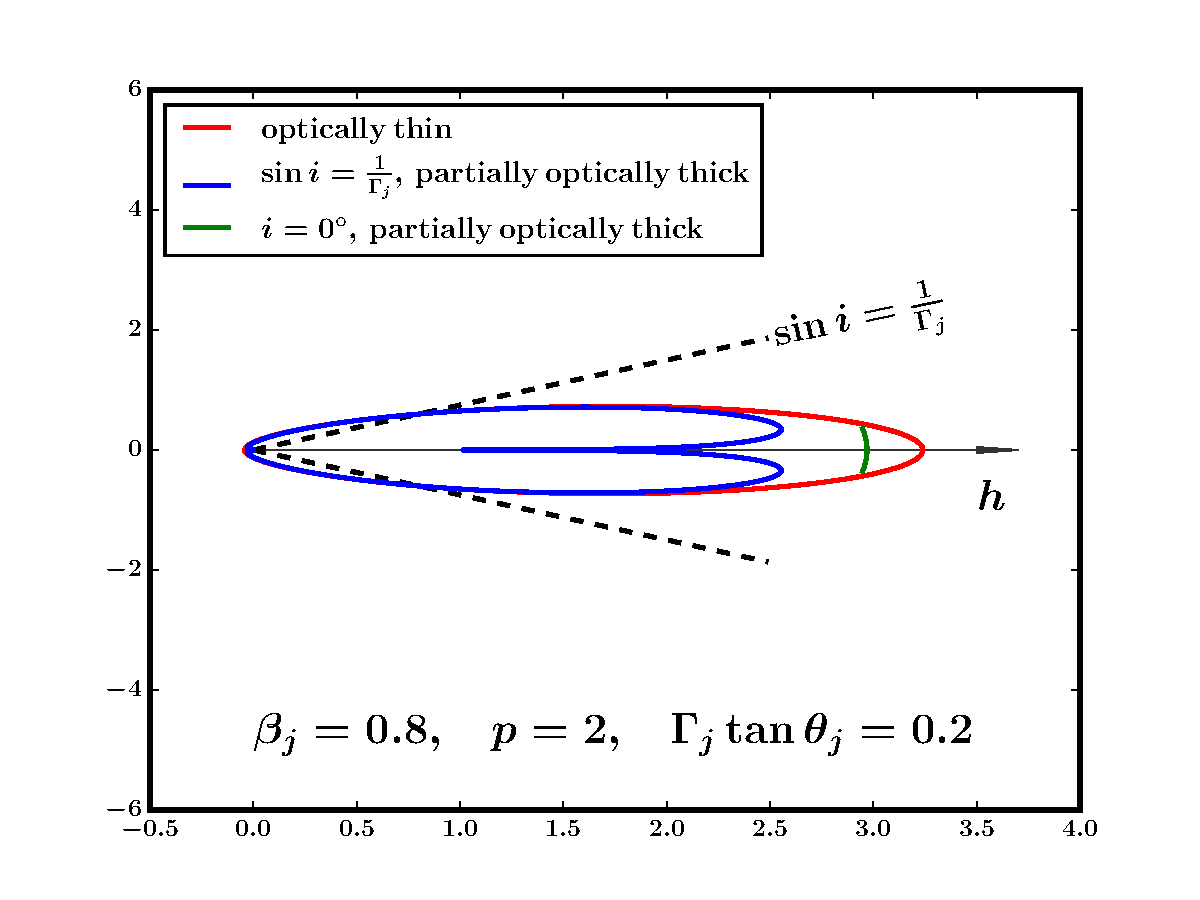
\includegraphics[scale=0.6]{beaming_final.pdf}\caption{The beaming pattern of the partially optically thick flux, shown for both small and large viewing angles for the fiducial parameters $ \beta_j = 0.8 $ and $ p = 2 . $ The flux when viewed on-axis is shown at angles smaller than the opening angle, defined as $ a \equiv \Gamma_j \tan \theta_j = 0.2 $ (see Section \ref{sec:comparison}), in green. The flux is normalized to unity at $ \sin i = 1 / \Gamma_j , $ which is Case (ii) in Fig. \ref{fig:The_emission_angles}. We can compare this to Fig. \ref{fig:beaming_initial}.}
\label{fig:beaming_final}
\end{figure}

We now solve for the countejet emission at low viewing angles. The LHS of Equation \ref{eq:full_radiative_transfer_jet} should now be multiplied by $ -1 $ since the photon path in the co-moving frame (which does not distinguish between jet and counterjet) is reversed. This, along with Equation \ref{eq:differential_optical_depth} yields
\begin{equation}
\dfrac{d}{d\tau}(I e^{\tau}) = S e^{\tau}, \label{eq:radiative_transfer_equation_for_counterjet}
\end{equation}
which is solved with the boundary condition that $ I = 0 $ at $ \tau = 0, $ i.e. at the observer. Again, the cross-section of the jet being independent of the optical depth, we can integrate the above Equation all the way to $ t(r) $ to obtain
\begin{equation}
I[t(r)] = e^{-t(r)} \intop_{0}^{t(r)} S(\tau^{'}) e^{\tau^{'}} d\tau^{'}, \label{eq:brightness_profile_of_counterjet}
\end{equation}
where $ t(r) $ is given by Equation \ref{eq:t_of_r}, which gives the required differential,
\begin{equation}
dI[t(r)] = S(\tau^{'}) e^{\tau^{'} - t(r)} d\tau^{'},
\end{equation}
which is then plugged into Equation  \ref{eq:flux_from_brightness}, include appropriate transformations, and include all the full range of $ \tau^{'} $ from $ 0 $ (because the upper parts contribute negligibly) to $ t(r) $  along the photon path, along with the transformations, to write
\begin{equation}
F_{cj} (i \sim 0) = \dfrac{2 \pi (1+z) \delta_{cj0}^3}{E_0 D^2} \int_{0}^{\infty} dr\, r \int_{0}^{t(r)} d\tau^{'} \, S(\tau^{'}) \exp[\tau'-t(r)],
\label{eq:counterjet_flux_integral}
\end{equation}
to give
\begin{equation}
F_{cj} (i \sim 0) = (1+z) \dfrac{ \alpha_f^{\frac{p-1}{p+4} } C_1 \tan ^2 \theta_j \; \delta_{cj0}^{\frac{3p+7}{p+4}} }{ 6 \left(\pi C_2 \right)^{\frac{p-1}{p+4}} (p+4)^{\frac{p+9}{p+4}} }\left(\dfrac{ \sigma_T h_0 K_0 B_{cr}}{B_0}\right)^{\frac{5}{p+4}} [ \cot{5\pi\over p+4} - \cot{\pi\over p+4} ] \dfrac{\Gamma\left(\frac{-4}{p+4}\right)}{\Gamma\left(\frac{1}{p+4}\right)} \frac{ c B_0{^2} }{\ee} \left(\frac{h_0}{D}\right)^2, \label{eq:Flux_counterjet_on_axis}
\end{equation}
where we remind ourselves that $ C_1 $ and $ C_2 $ depend on $ p . $

The total emission is, again, the sum of the fluxes from the jet and the counterjet.

We note that we have neglected here a possible (and likely in a range of angles) obscuration of the counterjet emission, by the accretion disc, stellar wind, and the jet in Microquasars, and the the dusty torus and the jet in blazars. The jet will actually reprocess the counterjet synchrotron emission, but this effect appears relatively minor.



\subsection{Viewed at large angles}

We note that Equation \ref{eq:Flux_counterjet_on_axis} with a replacement of $ \delta_{cj0} \rightarrow \delta_{j0} $ also gives the approximate jet emission at $ i' \sim 180 ^{\circ} $, which values of $ i' $ occur for most of values of $ i $ at large $ \Gamma_j , $ see Fig. \ref{fig:The_angle_transformation}. This formula can be then compared to Equation \ref{eq:Flux_side_view} at $ \Gamma_j \gg 1 , $ $ \sin i\sim 1 , $ see Section \ref{sec:comparison}.

In Fig. \ref{fig:beaming_final}, we show the solution of the problem showcased in Fig \ref{fig:beaming_initial}. In particular, the observed flux at low viewing angles does not go to null, but is higher than the maximum flux attainable in the side-view approximation.






\section{The relative jet flux at different angles} \label{sec:comparison}

In this Section, in reference to Fig. \ref{fig:beaming_final}, we compare the flux from the jet in the standard `side-view' approximation (see Case (ii) in Fig. \ref{fig:The_emission_angles}) to the small and large angles cases (Cases (i) and (iii) respectively).

The ratio of the jet flux in the on-axis view to the standard side-view flux is given by (Equations \ref{eq:Flux_jet_on_axis} and \ref{eq:Flux_side_view})
\begin{equation}
\frac{F_j (i \sim 0)}{F_j (i' \sim 90^{\circ})} = \dfrac{ \pi \, \Gamma \left( \frac{p-1}{p+4} \right) }{ C_3(p) \, (p+4)^{\frac{5}{p+4}} } \left[ \frac{\tan \theta_j}{\sin i} \right]^{ \frac{p-1}{p+4} } \left( \frac{\delta_{j0}}{\delta_j} \right)^{ \frac{3p+7}{p+4} }.
\end{equation}

In order to get a characteristic value of this ratio, we calculate it at $ \sin i = 1 / \Gamma_j . $ For that angle, $ \delta_{j0} / \delta_j = 1 + \beta_j . $ Then, we express the jet opening angle as a fraction of $ 1 / \Gamma_j , $ as $ a \equiv \Gamma_j \tan \theta_j . $ In theoretical models, often $ a = 1 $ is assumed \citep{Zamaninasab_et_al.-2014-Nature}, but observationally $ a < 1 $ is found. In particular, \citealt{Pushkarev_et_al.-2009-A&A} and \citealt{Clausen-Brown_et_al.-2013-A&A} found the average values in their samples of extragalactic jets of $ a \simeq 0.13 , \, \simeq 0.2 $ respectively. For jets in black-hole binaries, \citealt{Miller-Jones_et_al.-2006-MNRAS} also found $ a \ll 1 . $

Using the above relations, we obtain
\begin{equation}
\frac{F_j (i \sim 0)} {F_j ( i' \sim 90^{\circ} ) } = 
\dfrac{\pi \Gamma \left( \frac{p-1}{p+4} \right)}{C_3(p) \, (p+4)^{\frac{5}{p+4}}} a^{\frac{p-1}{p+4}}  ( 1 + \beta_j)^{\frac{3p+7}{p+4}}.
\end{equation}

We see that this ratio depends only on the fractional jet opening angle, $ a , $ the electron index, and $ 1 + \beta_j , $ which factor can assume values only between 1 and 2. We also see that this ratio is large unless $ a $ is very small. For example, for $ \beta_j \simeq 1 $ and $ p = 2 , \, 3, \, 4, $ it is $ \simeq  4.88 a^{1/6}, \; 5.73 a^{2/7} , \; 6.54 a^{3/7} $ respectively.


The ratio of the jet flux in the large-angle (Equation \ref{eq:Flux_counterjet_on_axis} with $ \delta_{cj0} \rightarrow \delta_{j0} $ ) view to the standard side-view flux is given by
\begin{equation}
\frac{F_j (i \sim 90^{\circ})}{F_j (i' \sim 90^{\circ})} = \dfrac{ 4 \pi^2 \, \Gamma \left( \frac{-4}{p+4} \right) }{ C_3(p) \, \Gamma \left( \frac{1}{p+4} \right) } [\cot \frac{5 \pi}{p+4} - \cot \frac{\pi}{p+4} ] \left[ \frac{\tan \theta_j}{\sin i} \right]^{ \frac{p-1}{p+4} } \left( \frac{\delta_{j0}}{\delta_j} \right)^{ \frac{3p+7}{p+4} }.
\end{equation}

For $ \sin i \sim 1 , $ this ratio becomes
\begin{equation}
\frac{F_j (i \sim 90^{\circ})}{F_j (i' \sim 90^{\circ})} = \dfrac{ 4 \pi^2 \, \Gamma \left( \frac{-4}{p+4} \right) }{ C_3(p) \, \Gamma \left( \frac{1}{p+4} \right) } [\cot \frac{5 \pi}{p+4} - \cot \frac{\pi}{p+4} ] \left[ \frac{a}{\Gamma_j} \right]^{ \frac{p-1}{p+4} } \left( {1 - \beta_j} \right)^{-\frac{3p+7}{p+4}}.
\end{equation}



\section{The jet-to-counterjet flux ratios} \label{sec:jet-to-counterjet_ratio}

We use the formulas of the observed flux in Cases (i), (ii) and (iii) of Fig. \ref{fig:The_emission_angles}, derived in the previous section, to obtain formulae for the jet-to-counterjet flux ratio in the side-view and on-axis view cases. We henceforth call this ratio $ R $, which can be used in conjunction with radio constraints, see \citealt{Stirling_et_al.-2001-MNRAS}, and estimates of inclination of the jet to the observer's line of sight, see \citealt{Orosz_et_al.-2011-ApJ}, to place constraints on the bulk speed of the jet.

For the case of side-view, in the low-energy regime (compared to the turn-over energy $ E_t  ), $ this can be simply read off Equation \ref{eq:Flux_side_view} to give
\begin{equation}
R = w^{-\frac{3p+7}{p+4}}. \label{eq:flux_ratio_side}
\end{equation}

The power-law index of this dependence changes from 2 for $ p = 1 $ to $ \simeq 3 $ for $ p \gg 1 $, different from the index of $ 2 $ for an optically thin jet with $ \alpha = 0 , $ and $ 3 $ for discrete plasmons (e.g. see T. V. Cawthorne's article in \citealt{Beams_and_jets}).

For the case of low viewing angles, Equations \ref{eq:Flux_jet_on_axis} and \ref{eq:Flux_counterjet_on_axis} need to be combined to give
\begin{equation}
R = w^{-\frac{3p+7}{p+4}} \, \frac{(p+4) \Gamma \left(\frac{1}{p+4}\right) \Gamma \left(\frac{p-1}{p+4}\right)}{4 \pi  \left[\cot \left(\frac{5 \pi }{p+4}\right)-\cot \left(\frac{\pi }{p+4}\right)\right] \Gamma \left(-\frac{4}{p+4}\right)} . \label{eq:flux_ratio_on-axis}
\end{equation}

We note that in general, the extra factor in this case does not deviate much from unity, e.g. it is $1.06275$ for $ p = 2 $ and $ 1.10463 $ for $ p = 3 , $ i.e. the deviation is $ \lesssim 10 \% . $ This means that it is safe to assume general validity of Equation \ref{eq:flux_ratio_side} and solve for $ \beta_j, $ to give

\begin{equation}
\beta_j=\frac{1}{\cos i} \dfrac{ R^\frac{p+4}{3p+7} - 1 }{ R^\frac{p+4}{3p+7} + 1 }.
\label{eq:beta}
\end{equation}




\section{The bulk Lorentz factor of Cygnus X-1} \label{sec:CygX-1}


\begin{figure}
\centerline{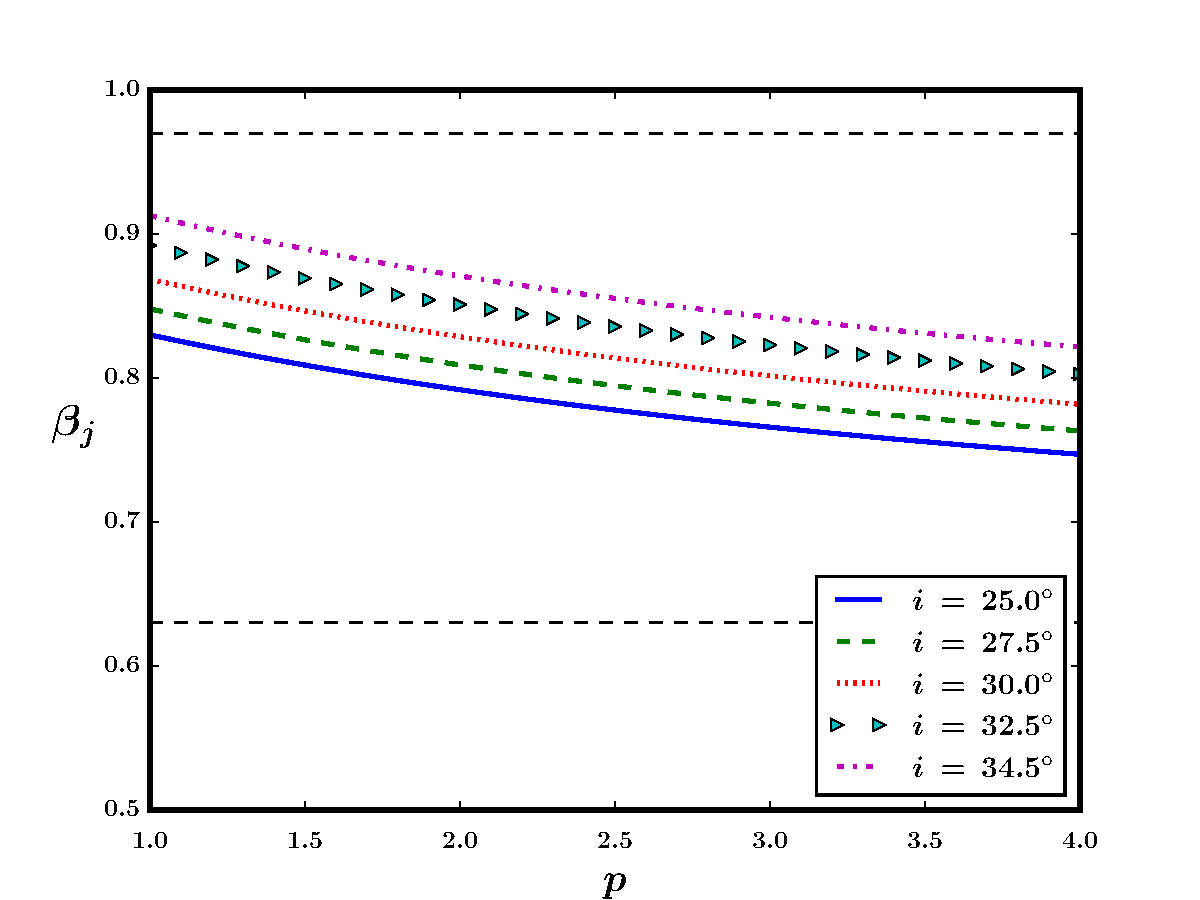
\includegraphics[scale=0.6]{beta_vs_p_CygX-1_Ziokowski.pdf}}
\caption{The lower limit on the velocity of the jet from Cyg X-1 as a function of the viewing angle, $ i , $ and the electron index, $ p . $ We use the range of the viewing angles found by \citealt{Ziolkowski-2014-MNRAS} and the lower limit on the ratio of the jet-to-counterjet flux ratio obtained by \citealt{Stirling_et_al.-2001-MNRAS} of $ R \geq 50 . $ The horizontal lines correspond to the previous limits given in their Table 2.
}
\label{eq:beta_p}
\end{figure}


\citealt{Stirling_et_al.-2001-MNRAS} have obtained radio maps of the black-hole binary Cyg X-1 using VLBA and VLA at 8.4 GHz. They have found no evidence for the presence of a counterjet, and constrained the flux ratio to $ R \gtrsim 50 $. They assumed $ i = 40^{\circ} $ and optically-thin emission in calculating constraints on the jet velocity. Currently, a lower value of $ i $ appears to be the inclination of the orbit of Cyg X-1, in particular \citealt{Orosz_et_al.-2011-ApJ} found $ i \simeq 27 \pm 1 ^{\circ} . $ On the other hand, \citealt{Ziolkowski-2014-MNRAS}, considering also the evolutionary status of the system, found $ i \simeq {29^{+5}_{-4}}^{\circ} $ as the most likely range. For this range, Equation \ref{eq:beta} at $ p = 2 $ gives $ \beta_j \geq 0.82_{-0.03}^{+0.05} , $ corresponding to $ \Gamma_j \geq 1.75_{-0.11}^{+0.25} . $ A caveat for this result is that the jet is likely aligned with the black-hole rotation axis, which may be misaligned with the normal to the binary plane. In this case, the jet inclination may be not given by the above constraints.

Other constraints on the jet velocity in Cyg X-1 are by \citealt{Gleissner_et_al.-2004-A&A}, who claimed $ \beta_j \lesssim 0.7 $ based on non-detection of short-time scale correlations between radio and X-ray emission, though this limit appears model-dependent. Then \citealt{Malzac_Belmont_Fabian-2009-MNRAS}, estimated $ 0.3 \lesssim \beta_j \lesssim 0.8 , $ which again relies on a number of assumptions.

\citealt{Stirling_et_al.-2001-MNRAS} also constrained the half-opening jet angle of the projection of the jet on the sky as $ \lesssim 2^{\circ} . $ We note here that the actual half-opening angle is the one after de-projection, i.e., multiplied by $\sin i$ \citep{Konigl-1981-ApJ}. Given that $ i \simeq 30 ^{\circ} , \; \theta_j \lesssim 1 ^{\circ} . $ Since the lower limit on $ \Gamma_j $ is rather low, this upper limit on the half-opening angle implies a very small factor $ a \equiv \Gamma_j \tan \theta_j , $ unless $ \Gamma_j $ is much higher than the lower limit of \citealt{Stirling_et_al.-2001-MNRAS} obtained from the absence of an observed counterjet. If $ \Gamma_j = 2 , a \lesssim 0.035 . $ This coefficient is substantially lower than those typically seen in blazars, where $ a \simeq 0.2 $ \citep{Clausen-Brown_et_al.-2013-A&A}.


\section{Conclusions} \label{sec:conclusions}

We have studied the extended synchrotron jet model, originally proposed by \citealt{Blandford_&_Konigl-1979-ApJ}. We have considered three limiting analytical approximations to the flux vs.\ the viewing angle. In one, usually assumed, the jet is viewed sideways in the comoving frame. This approximation implies that the flux becomes null when the jet is viewed on axis, with $ i \simeq 0 , $ e.g., T. V. Cawthorne's article in \citealt{Beams_and_jets}. However, we point out that the above approximation breaks down in the low-$ i $ regime, since the jet is no longer viewed sideways in the comoving frame. We have considered another limiting case, of the jet viewed on axis. We have found an analytical solution of the radiative transfer integrated over the jet cross section in that case. We have found out that this emission is rather strong, corresponding to the global maximum of the flux as a function of the viewing angle. 

We have also calculated the emission corresponding to the jet-frame emission angle of $ i' \sim 180^{\circ} .$ This regime corresponds to the viewing angles of $ i \gg 1/\Gamma_j $ when the jet bulk Lorentz factor, $ \Gamma_j , $ is large. This case also corresponds to the counterjet emission in the case of $ i \simeq 0 . $

We have applied our results to the black-hole binary Cyg X-1. Given the jet-to-counterjet flux ratio of $ \gtrsim 50 $ found observationally \citealt{Stirling_et_al.-2001-MNRAS} and the current estimate of the inclination of $ i \simeq {29^{+5}_{-4}}^{\circ}$ \citealt{Ziolkowski-2014-MNRAS}, we have found $ \beta_j \gtrsim 0.8 , $ $ \Gamma_j \gtrsim 1.6 . $ We have also pointed out that when the projection effect is taken into account, the radio observations imply the jet half-opening angle of $ \theta_j \lesssim 1^{\circ} , $ a half of the value given by \citealt{Stirling_et_al.-2001-MNRAS}. If $ \Gamma_j $ is not much above the counterjet limit, the opening angle is $ \theta_j \ll 1/\Gamma_j , $ and much lower than the values typically observed in blazars.



\section{Discussions} \label{sec:discussions}

In this chapter, we have addressed two key questions:
\begin{enumerate}
\item How robust is the current procedure to estimate the speed of `continuous' jets?
\item What is the anisotropy of continuous partially self-absorbed synchrotron jets?
\end{enumerate}

Answers to the above questions are obtained:
\begin{enumerate}

\item The parametrization of the present method is poorly understood, and our thorough theoretical analysis allows it to be understood as well as improved. A more robust formula is provided, and demonstrated for Cygnus X-1 in Section \ref{sec:CygX-1}. However, it is noted that the proposed formula also depends on an independent measurement of the inclination angle (or `viewing angle') of the jet, which although in general difficult, can be indirectly measured through binary inclinations for black hole binary systems like Cygnus X-1.

\item A more difficult question, a complete answer could not be obtained within the scope of this work. However, breaking the problem into parts offer insights that are in general either ignored or not explicitly mentioned, but found here to be important. The effects of special relativity, with no counterparts in classical mechanics, are found to be strongly affecting the observation of relativistic jets.

\end{enumerate}

There are several assumptions, caveats and limitations in the work presented in this chapter, other than those already mentioned. Whereas not all the assumptions may be applicable to particular systems, the limitations need to be addressed by more detailed studies, in different directions. Below we list a few of the limitations, and propose directions for a deeper understanding of the subject of astrophysical jets:

\begin{enumerate}

\item We do not study the `central engine' of jets, the source of energy of relativistic particles that finally radiate the observed energy. A reasonable assumption is that the central engine is the inflowing matter into the central compact object, either in an accretion disk (\citealt{Shakura_&_Sunayev-1973-AAp}) or spherically symmetric Bondi flow (\citealt{Bondi-1952-MNRAS}). However, we probe the jet at length-scales much larger than the gravitational radius of the compact object (see \citealt{Zdziarski-2012-MNRAS-Radio_modulation_CX1}, \citealt{Zdziarski_et_al.-2012-MNRAS-MeV_tail_CX1}), and the central engine is assumed to not play a crucial role at these lengths.

\item Although we consider only 'steady' jets, like that of Cygnus X-1 in its hard spectral state (see \citealt{Stirling_et_al.-2001-MNRAS}, \citealt{Zdziarski-2012-MNRAS-Radio_modulation_CX1}) some recent studies (see \citealt{Gandhi_et_al.-2011-ApJ}) claim to be probing variability of the base of the steady jets of Microquasars. Although the findings are debatable, we note that no jet can be perfectly steady, and in general the variability is not being observed because the intrinsic variability is washed out over observational time-scales, presenting an average picture of the jet. The relevant variability time-scales are those related to the central engine itself, the physical processes that govern the transfer of energy into the particles and the radiation processes. This can be addressed by simulations of the energy source, e.g. as those done in the internal shock model for the case of blazars by \citealt{Joshi_&_Bottcher-2007-ApJ} and Microquasars by \citealt{Jamil_et_al.-2010-MNRAS}. These studies suffer from internal inconsistencies, and a full understanding involving the full microphysics in all scenarios is yet to be emerge. Moreover, jets are known to be highly variable across wavelengths, in blazars \citep{Kushwaha_et_al.-2013-MNRAS,Agarwal_et_al.-2015-MNRAS,Agarwal_et_al.-2016-MNRAS} and in the soft state of Microquasars (\citealt{Mirabel_&_Rodriguez-1994-Nature}), and this aspect is beyond the scope of the present work.

\item We do not discuss what fraction of the jet power is radiatively efficient, and what fraction is only the kinetic. Some studies, like \citealt{Heinz-2006-ApJ}, \citep{Gallo_et_al.-2005-Nature} and \citealt{Malzac_Belmont_Fabian-2009-MNRAS}, address this issue.

\item We assume that the particle population is leptonic, and do not discuss the composition of jets. We note that the question is observational. Even in the observational front, it is a difficult topic, except in the case of blazars, where the lepto-hadronic (see \citealt{Sahayanathan_&_Godambe-2012-MNRAS}) model is more favoured over purely hadronic model (see \citealt{Paliya_et_al.-2016-arXiv}), although there is no clear case against either.

\item The deceleration of the large-scale jets, as the particle-population become non-relativistic, or stop radiating, is not discussed in this work. The finiteness of the height of the jet affects the very low-energy part of the spectrum, which is currently not probed observationally, does not affect our results. This topic can be studied via simulation of jets, tracking the particle-distribution in both the energy-space and spatial scales.

\item The energy-scale in the problem is kept free, in this study. It can be probed by observations, and physically, the `jet-base' defines where the `turnover' energy should lie. In the case of Microquasars, the situation is complicated by the presence of the donor star, e.g. in Cygnus X-1, in which although \citealt{Rahoui_et_al.-2011} claim to have estimated the turn-over energy, is a highly debatable result. Such debates can be addressed by broadband spectral modelling that takes into account the jet-contributions. The SED modelling of both blazars (\citealt{Joshi_&_Bottcher-2007-ApJ}, \citealt{Paliya_et_al.-2015-ApJ}) and Microquasars (\citealt{Zdziarski_et_al.-2014_b-MNRAS}) shows the presence of a wide range of  components arising from the black hole environment.  We note that such studies should carefully take into account the synchrotron cooling of the particle spectrum, and also the synchrotron self-comptonization, both affecting the high energy spectrum of astrophysical systems. We point out that our analysis removes the internal inconsistency in the model of \citealt{Zdziarski_et_al.-2014_a-MNRAS}, in which the speed of the jet and the power-law index are assumed to be independent, and an interesting future endeavour is to remove this inconsistency numerically, which is however not pursued here. Although simultaneous multi-wavelength coverage of some systems are available from Astrosat, GMRT and NICS, the absence of data in the sub-mm, NIR, and FIR limits the estimation of the energy-scale in the problem.

\item Synchrotron radiation from a single particle is polarized. Since the polarization of a particle-distribution is dependent on the geometry of the magnetic fields, the polarization properties of the observed radiation probe the geometry as well as magnitude of the magnitude of the magnetic fields in the jet, which are otherwise difficult to constrain because of the presence of too many parameters in the problem. Moreover, in our model, the magnetic field is assumed to be tangled in the jet-frame, which predicts zero observed polarization. However, in the \citealt{Blandford_&_Konigl-1979-ApJ} model, the magnetic field profile is set by the conservation of energy, and is applicable also to the case of toroidal magnetic fields. So it will be an interesting future endeavour to calculate the polarization fraction from our model, only making the magnetic fields toroidal, which does not affect the present results. Moreover, making polarization maps for both Microquasars and AGN can throw light on the geometry of the fields. This, in turn, can be used in removing degeneracies in the broadband modelling.

\item The beaming pattern of synchrotron jets can be extended to study the beaming of afterglows in Gamma Ray Bursts and the more enigmatic Fast Radio Bursts, not pursued here due to the presence of other complications in these sources that are poorly understood.

\end{enumerate}

Despite the several assumptions, caveats and limitations in our study, we try to emphasize the importance of reviewing `standard' models, and questioning `established' results. We wish to point out that to answer the more challenging and intricate questions related to astrophysical jets, the simplest ideas need to be understood thoroughly, which can offer new insights. We hope that our work provides a stepping stone to future studies, both generic and specific.






















%\bibliographystyle{apj}
%\bibliography{debdutta}
%
%
%\end{document}